\documentclass{article}

\usepackage{amsmath}				% American Mathematical Society
\usepackage{amssymb}

\usepackage{tikz}

%-------------------------------------------------------
%: xmin xmax ymin ymax
\tikzset { xmin/.store in=\xmin, xmin/.default=-3, xmin=-3,
           xmax/.store in=\xmax, xmax/.default=3, xmax=3,
           ymin/.store in=\ymin, ymin/.default=-3, ymin=-3,
           ymax/.store in=\ymax, ymax/.default=3, ymax=3}

%: domaine
\tikzset {domaine/.style 2 args={domain=#1:#2}}

%: Commande \grille : trace la grille entre (xmin,ymin) et (xmax,ymax)
\newcommand {\grille} {\draw[help lines] (\xmin,\ymin) grid (\xmax,\ymax);}

%: Commande \axes
\newcommand{\axes}
{\draw[->] (\xmin,0) -- (\xmax,0); \draw[->] (0,\ymin) -- (0,\ymax);}

%: Commande \fenetre : limite de l'affichage  (xmin,ymin) et (xmax,ymax)
\newcommand {\fenetre} {\clip (\xmin,\ymin) rectangle (\xmax,\ymax);}

%-------------------------------------------
\begin{document}

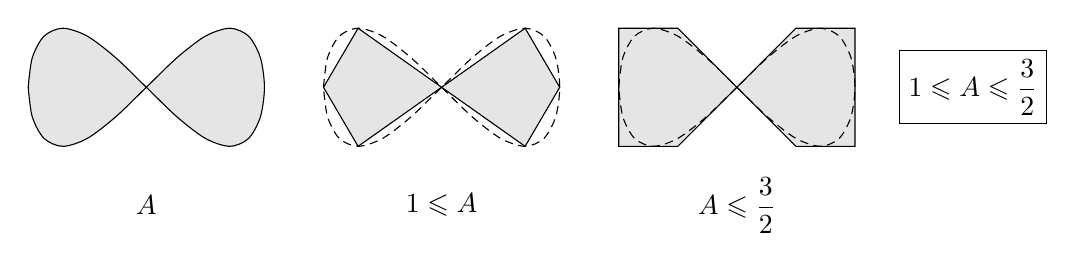
\begin{tikzpicture}[scale=1.5]
  % figure 1
  \begin{scope}
    \filldraw[fill=gray!20]   % la courbe et l'aire
      plot [smooth,domaine={-pi}{pi}] ({cos(\x r)},{cos(\x r)*sin(\x r)});
    \draw (0,-1) node {$A$};  % commentaire
  \end{scope}
  % figure 2
  \begin{scope}[xshift= 2.5cm]
    \draw[fill=gray!20] (0,0) -- ({sqrt(2)/2},0.5)
      -- (1,0) -- ({sqrt(2)/2},-0.5) -- ({-sqrt(2)/2},0.5)
      -- (-1,0) -- ({-sqrt(2)/2},-0.5) -- cycle;
    \draw[densely dashed]
      plot [smooth,domaine={-pi}{pi}] ({cos(\x r)},{cos(\x r)*sin(\x r)});
    \draw (0,-1) node  {$1\leqslant A$};  % commentaire
  \end{scope}
  % figure 3
  \begin{scope}[xshift= 5cm]
    \draw[fill=gray!20] (0,0) -- (0.5,0.5) -- (1,0.5)
      -- (1,-0.5) -- (0.5,-0.5) -- (-0.5,0.5)
      -- (-1,0.5) -- (-1,-0.5) -- (-0.5,-0.5) -- cycle;
    \draw[densely dashed]
      plot [smooth,domaine={-pi}{pi}] ({cos(\x r)},{cos(\x r)*sin(\x r)});
    \draw (0,-1) node  {$ A\leqslant \dfrac{3}{2}$};  % commentaire
  \end{scope}
  % commentaire
  \begin{scope}[xshift= 7cm]
    \draw (0,0) node  {\fbox{$1 \leqslant A \leqslant \dfrac{3}{2}$}};
  \end{scope}
\end{tikzpicture}

\end{document}
